\chapter{System Design and Overview}
\label{cha:4th_chapter}

The purpose of this chapter is to give a detailed description of how we optimized the input pipeline (Section \ref{sec:input_pipeline}) of our models and how we built the architecture of the networks used (Section \ref{sec:nn_architecture}) in this work. 
In Section \ref{sec:training} we present details from the training algorithm and which are the losses used in the update step, while Section \ref{sec:evaluation_metrics} illustrates the evaluation metrics the we used in order to have a quantitative measure of how good were performing the trained networks.

\section{Input Pipeline}
\label{sec:input_pipeline}
After preprocessing the dataset with the transformations described in Section \ref{sec:preprocessing} (cropping and normalization), we proceeded to store the data as a \textit{TFRecord}. 


TFRecord, provided with the free and open-source software library of \textit{Tensorflow}, is a format that allows large amount of data to be read in an efficient way \cite{tfrecord} by serializing it and storing it as a sequence of binary records of varying sizes:~\ac{GPU}s, together with an efficient input pipeline (that starts from choosing the right data format), allow to achieve peak performance and to reduce computational times.

\vspace{2mm} %5mm vertical space
In order to build an highly performant input pipeline for the models we applied some important operations to our TFRecord data including a preprocessing step on the fly while loading data with the \textit{Data API}:

\begin{itemize}
\item \textbf{Caching} the dataset in memory to save operations, such as file opening and data reading, from being executed during each epoch. It was crucial to apply this step before shuffling, batching and prefetching: data is read only once but is shuffled (next step) every time in a different way, with the next batch still being prepared in advance \cite[p.~915]{hands_on_ml}.
\item \textbf{Shuffling} the training set (with buffer size set to 128) since \textit{Gradient Descent} works best when the instances are independent and identically distributed.
\item We then performed \textbf{Mapping} to decode efficiently the binary information and store it into tensors. Inside this step, another processing transformation was applied to the data: a constant (zero - value) padding was added to images to reshape them as [256, 256, 128], i.e., a shape compatible with the input generator of the~\ac{GAN}s implemented (see Section \ref{sec:nn_architecture} for more details). 
\item \textbf{Batching} plays a major role in the training of deep learning models and because of this it was crucial to choose the right batch size based on the~\ac{GPU} available and on the neural networks that we were going to train. 

Choosing the right batch size is important because it determines how many images are used to train the model before updating all the weights and biases. In our case we identify, after performing various experiments varying the batch size from 1 to 256, that 32 was the right number of images to use, at each iteration of the training algorithm, as input for all the models implemented.

\vspace{2mm} %5mm vertical space
\begin{table}[htbp!]
\centering
\begin{tabular}{ccc}
\toprule
Batch size & Batches/epoch & Train time/epoch (s)\\
\midrule
1 & 1024 & $\approx500$\\
4 & 256 & $\approx130$\\
8 & 128 & $\approx75$\\
16 & 16 & $\approx40$\\
\textbf{32} & \textbf{32} & $\mathbf{\approx30}$\\
64 & 16 & $\approx25$\\
128 & 8 & $\approx23$\\
256 & 4 & GPU out of memory\\

\bottomrule	
\end{tabular}
\captionsetup{justification=centering}
\caption[Train time/epoch of pix2pix using a reduced set of 1024 images]{Train time/epoch of pix2pix using a reduced set of 1024 images.}
\label{tab:batch}
\end{table}

Table ~\ref{tab:after_norm} shows some of the experiments we performed to determine the proper batch size, evaluating the training time taken by pix2pix (Subsection \ref{subsec:pix2pix_architecture}) on~\ac{GPU} with a reduced dataset of 1024 images, varying the size of the batch and consequently the number of batches.
     
\vspace{2mm} %5mm vertical space
We noticed that a batch size equal to 256 couldn't fit the~\ac{GPU} RAM provided by Google Colaboratory: the processors were running out of memory giving an error of resource exhausted.
Furthermore, even though the training time was slower with respect to the times obtained with batch size of 64 and 128, we observed that 32 reached, qualitatively, more accurate results in the generated samples and \cite[p.~681]{hands_on_ml} explains the reason: in practice, large batch sizes often can lead to training instabilities and so the models may not generalize as well as a model trained with smaller batch size. 

\item Finally we applied a \textbf{Prefetching} step to have the preprocessing overlapping with the training execution: while the model is executing training step \textit{s}, the input pipeline is saving time by reading data that will be used in the next training step \textit{s+1}.

\end{itemize}

\begin{figure}
\centering
\includegraphics[height=0.40\textheight]{images/batch.pdf}
\caption[A batch from training set: 32 $T_{1}$ processed slices]{Example of single channel batch from the training set, with 32 $T_{1}$ slices cropped, normalized, shuffled and padded, with dimensions 256x256, ready to be fed to a single input model.}
\label{fig:batch}
\end{figure}

\section{Neural Networks Architecture}
\label{sec:nn_architecture}
In this work we developed two Generative Adversarial Networks: a multi-input version of pix2pix\cite{pix2pix}, that we called MI-pix2pix, and a modified version of the MM-GAN proposed by Sharma et al. in\cite{migan}.
We also implemented pix2pix that was used mainly as a baseline to compare the performances reached by our multi-modal \ac{GAN}s, to see if they were producing better results, both in a qualitatively and quantitatively way.

\vspace{2mm} %5mm vertical space
In this section we discuss in detail the architectures behind these three~\ac{GAN}s, showing also the differences between the model proposed by Sharma et al. and our modified version.

\subsection{Pix2pix}
\label{subsec:pix2pix_architecture}
Pix2pix is a single input - single output~\ac{GAN}, proposed by Isola et al. in \cite{pix2pix} as a solution to the problem of image-to-image translation, extensively discussed in Subsection \ref{subsec:image-to-image_translation}.
This Generative Adversarial Network adopts a modified U-Net architecture\cite{unet} as generator and a PatchGAN\cite{patchgan} as discriminative model that tries to distinguish between the true samples coming from the dataset and the synthesized images of the generator.

\vspace{6mm} 
\noindent\textbf{Generator}

\vspace{2mm}
\noindent In Subsection \ref{subsec:image-to-image_translation} we discussed about the strength of U-Net as generative network: skip connections between mirrored layers that represent a solution to the problem of losing information through the bottleneck layer. These connections are realized linking the \textit{i} layer to the \textit{n-i} layer (where \textit{n} is the total number of layers) that receives as input a concatenation between the output of the \textit{i} layer and the information processed by the \textit{n-(i+1)} layer.

\vspace{2mm} %5mm vertical space
The generator architecture, with the U-shape from which U-Net takes its name, is illustrated in Figure~\ref{fig:pix2pix_generator}. The input of the model is a tensor with size 32x256x256x1, where the first one indicates the batch size, so how many images are used per time for a single update. 

\begin{figure}[H]
\centering
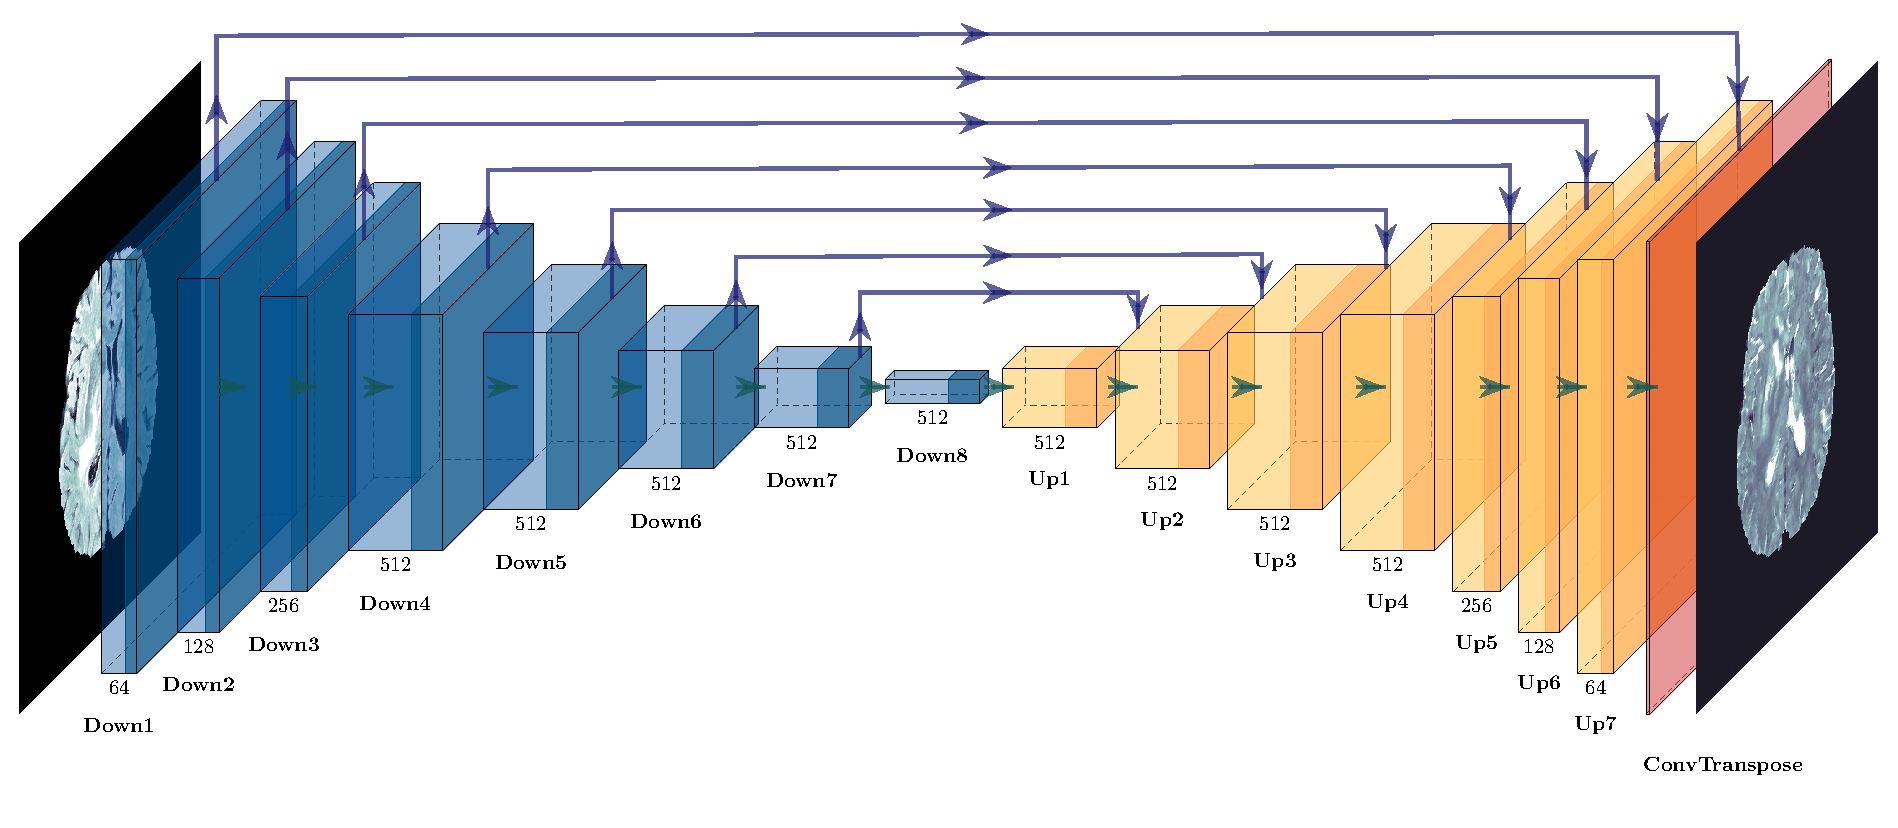
\includegraphics[height=0.266\textheight]{images/pix2pix_generator.pdf}
\caption[Generator architecture from pix2pix]{Generator architecture from pix2pix \cite{pix2pix}.}
\label{fig:pix2pix_generator}
\end{figure}

In Section \ref{sec:input_pipeline} we explained that it was necessary to add a padding to our images because otherwise they wouldn't have been compatible to the input of the images: the problem with U-Net comes from the nature of its mirrored architecture and more in particular from its downsampling and upsampling layers that allow to have only input images with dimensions that are power of 2. We choose then to pad our 180x180 images in order to obtain a width and height of 256, instead of applying a resize/crop to 128: transformation that wouldn't have preserved all the information in the images. 

\vspace{2mm} %5mm vertical space
The input fed to the model goes first through the contracting path: a typical convolutional neural network (Subsection \ref{sec:convolutional_neural_network}) composed by the repeated application of one the two main building blocks of the network, the \textbf{downsample block}, composed as follows:

\begin{itemize}
\item \textbf{Convolution}, that halves the dimensions of the input by convolving it through several filters with a fixed kernel size equal to 4 and stride of 2 for all the spatial dimensions.
\item \textbf{Batch Normalization} in every block (with the exception of the first one). This operations zero-centers and normalizes each input, trying to overcome to the problem of the vanishing gradient \cite[p.~728]{hands_on_ml}.
\item \textbf{Leaky ReLU}, an activation function similar to ReLU but with a small slope for negative values useful to avoid that some neurons "die" during training (meaning that they stop outputting anything other than 0) \cite[p.~720]{hands_on_ml}.
\end{itemize}
The repeated downsampling reduces the spatial information while increases the feature dimension, until the input arrives at the bottleneck where the output shape of the last downsampling block (\textit{Down7}) is [1x1x512].

\vspace{2mm} %5mm vertical space
The building block that characterizes the expanding path of the network is instead the \textbf{upsample block}, composed by four layers:

\begin{itemize}
\item \textbf{Transposed convolution} that goes in the opposite direction of what is done by the Convolution, by enlarging the spatial information: image is first stretched with the insertion of empty rows and then a regular convolution is computed. A kernel size of 4 and stride of 2 was set in this layer.
\item \textbf{Batch Normalization}
\item \textbf{Dropout}, useful for its regularization effect against some possible overfitting, it was applied in the first three upsampling blocks.
\item \textbf{ReLU} that has the advantage to not saturate for positive values (and it is fast to compute) \cite[p.~720]{hands_on_ml}
\end{itemize}

The last layer in the architecture of the generative part of \cite{pix2pix} is another transposed convolution that prepares the output of the model with tanh (hyperbolic tangent) as activation function, that returns values in a range between -1 and +1.
The output of the network is a batch of images, 32 in our case, with dimension 256x256x1.

\vspace{6mm} 
\noindent\textbf{Discriminator}

\vspace{2mm}
\noindent The PatchGAN \cite{patchgan} used to distinguish true images from fake images is similar to the well-known Convolutional Neural Network architecture (Section \ref{sec:convolutional_neural_network}), with the difference that the discriminator of pix2pix doesn't discriminate the whole image but small \textit{N}x\textit{N} patches of the input image: in this way the network can focus on capturing high frequencies details and assign to each patch a fake or true label. 

This means that the output of the discriminator we used, in pix2pix and in the other \ac{GAN}s we experimented with, isn't a 1x1 value but a 30x30 matrix, where each value contains the result of the discrimination over a 70x70 portion of the input image (the authors that developed \cite{pix2pix} suggest to use a patch of this size to obtain the best results from the \ac{GAN}).

\vspace{2mm} %5mm vertical space
Because of this, the network used is called 70x70 PatchGAN and takes two inputs, as illustrated in Figure~\ref{fig:pix2pix_discriminator}, each with shape [32, 256, 256, 1]: the first one is an input image while the second one is the target that can be an image coming from the dataset or a sample  generated by the \ac{GAN}. 

\begin{figure}[H]
\centering
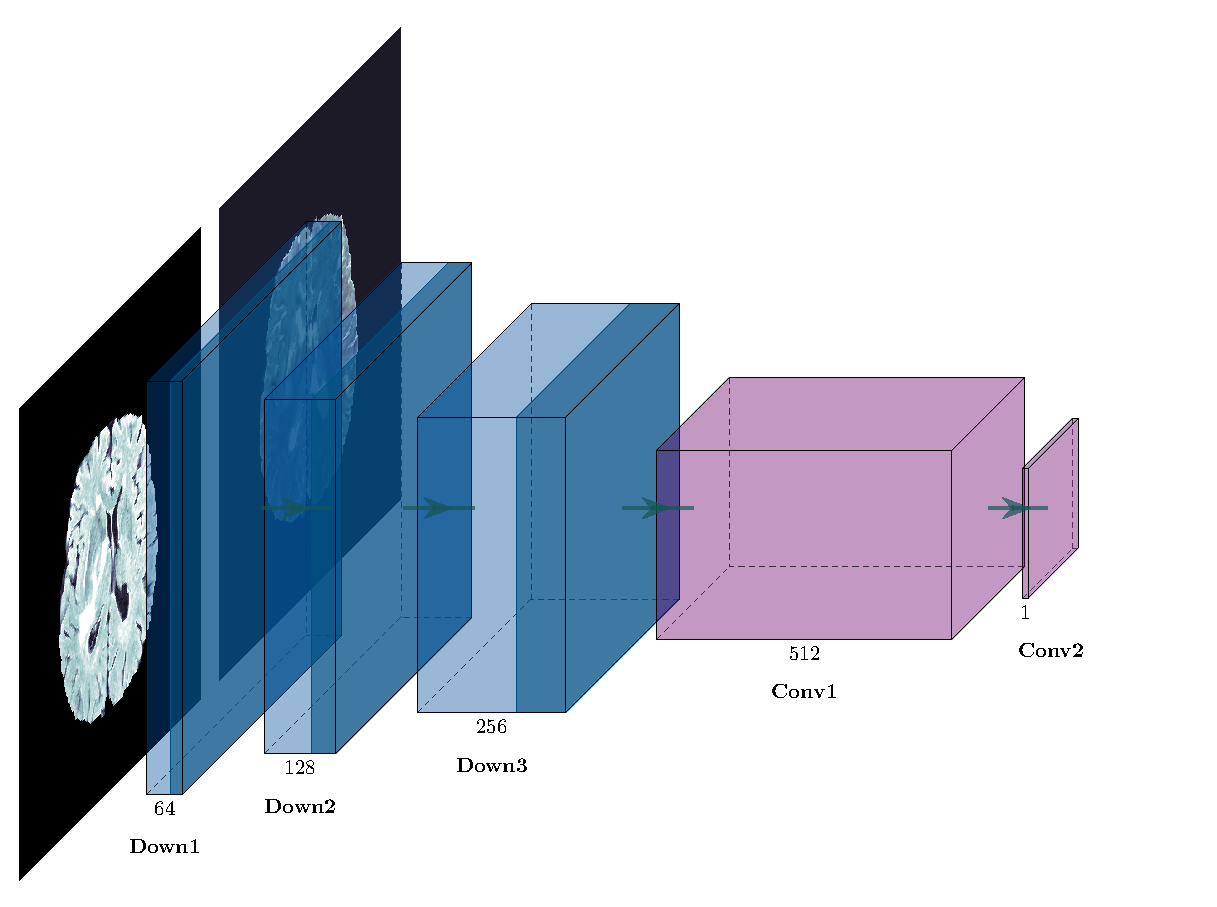
\includegraphics[height=0.3\textheight]{images/pix2pix_discriminator.pdf}
\caption[Discriminator architecture from pix2pix]{Discriminator architecture from pix2pix \cite{pix2pix}.}
\label{fig:pix2pix_discriminator}
\end{figure}

\vspace{2mm} %5mm vertical space
The discriminator architecture, differently from the one of the generator, has only a contracting path and is composed by three downsample blocks that allow to reduce the spatial dimensions of the image while increasing the feature dimension. Each one of these blocks is characterized by a different number of filters (64 the first block, 128 the second one and 256 the last one) and they are defined with the same layers that compose a downsample block in the generator (so batch normalization applied only in \textit{Down2} and \textit{Down3}.


These blocks are then followed by several layers: 

\begin{itemize}
\item \textbf{Zero Padding}, that doesn't increment the number of trainable parameters, because it simply adds zeros at the top, left, right and bottom of an image.
\item \textbf{Convolution} with 512 filters, kernel size equal to 4 and stride of 1.
\item \textbf{Batch Normalization}
\item \textbf{Leaky ReLU}
\item \textbf{Zero Padding}
\item Final \textbf{convolution} with 1 filter, again with kernels of 4x4 and stride set to 1.
\end{itemize}

\noindent The description of the training algorithm used by pix2pix can be found in Subsection \ref{subsec:training_algorithm} while the implementation details are discussed in Subsection \ref{subsec:implementation_details}.

\subsection{MI-pix2pix}
\label{subsec:mi_pix2pix_architecture}
MI-pix2pix is the second Generative Adversarial Network that we included in our experiments: it is a modified version of pix2pix \cite{pix2pix} adapted to a multi-input scenario in order to compare and evaluate the differences between an unimodal approach and its variant that takes multiple modalities of available information as input.

\vspace{6mm} 
\noindent\textbf{Generator}

\vspace{2mm}
\noindent The layers that compose the generator architecture (Figure~\ref{fig:MIpix2pix_generator}) are the same as the ones that define the pix2pix model with the only difference in the input shape, that is set to [32, 256, 256, 3], while the output shape remains equal to [32, 256, 256, 1]. For example a MI-pix2pix that has to synthesize the missing $T_{2}$ sequence of a subject will use the information from the other three modalities available: $T_{1}$, $T_{1c}$, $T_{flair}$ that are the inputs respectively of the first, second and third input channel.

\vspace{6mm} 
\noindent\textbf{Discriminator}

\vspace{2mm}
\noindent Also for the Discriminator we maintained the same architecture (Figure~\ref{fig:MIpix2pix_discriminator}) used in the unimodal version of pix2pix, but, since we are in a multi-modal setting, while the target has still a shape of [32, 256, 256, 1], the second input is a concatenation of the three modalities ([32, 256, 256, 3]) used to feed also the Generator.

\begin{figure}[H]
\centering
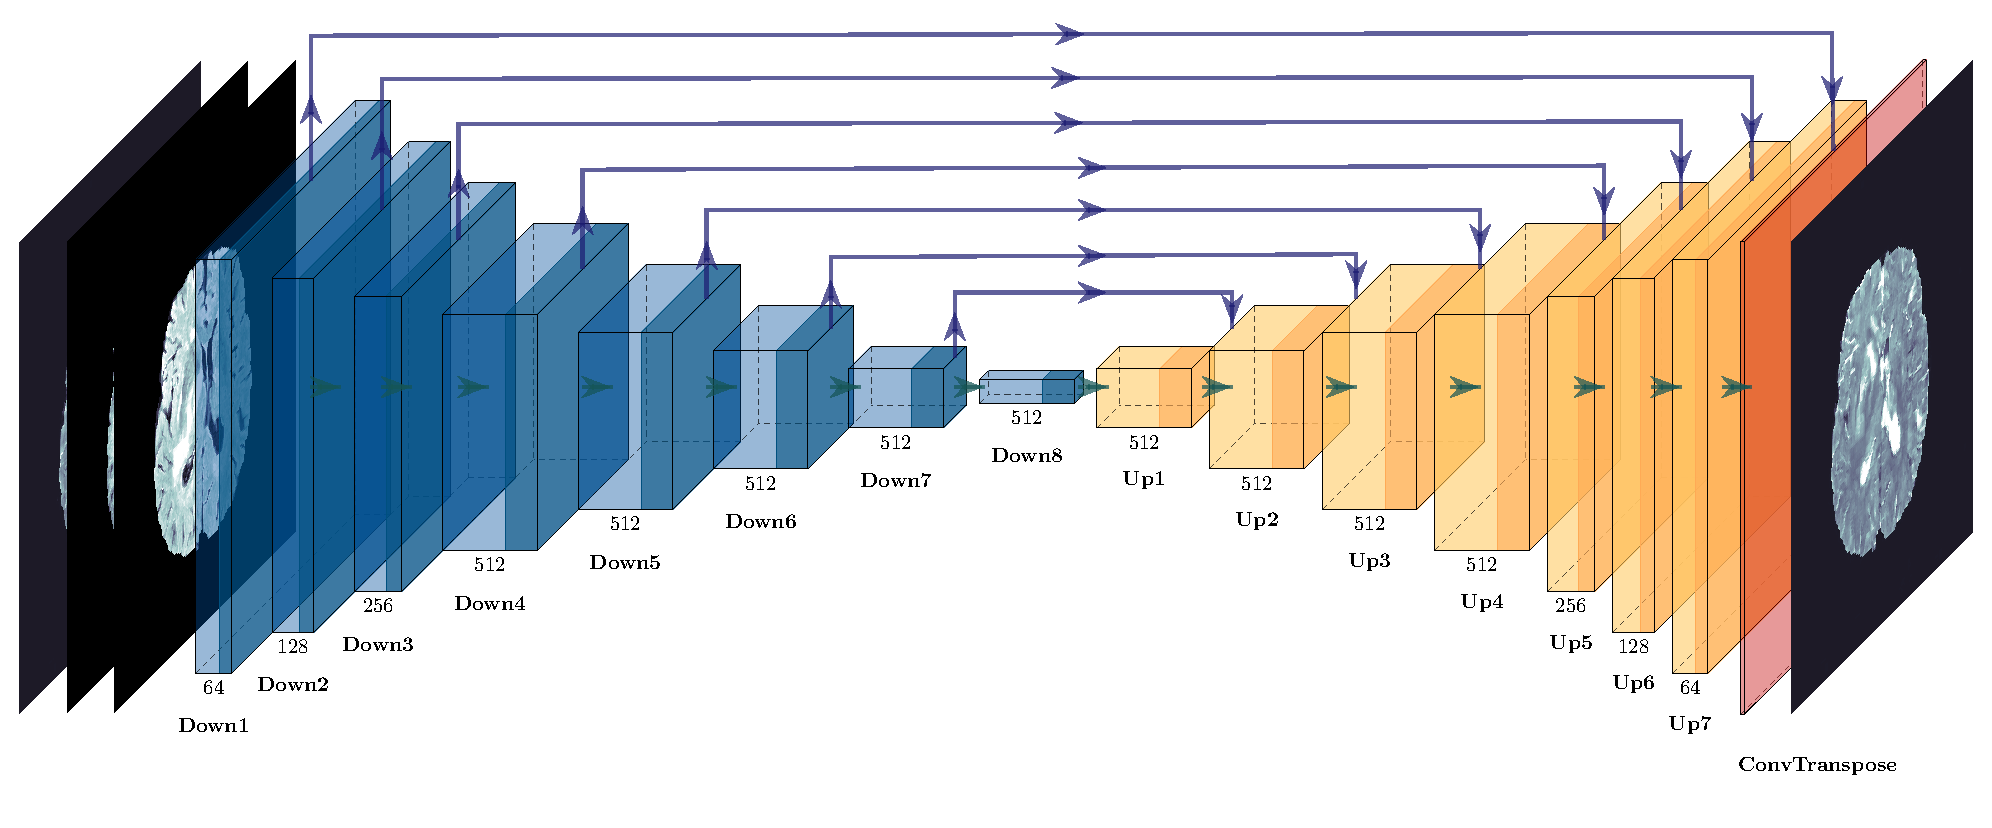
\includegraphics[height=0.263\textheight]{images/MIpix2pix_generator.pdf}
\caption[Generator architecture from MI-pix2pix]{Generator architecture from MI-pix2pix.}
\label{fig:MIpix2pix_generator}
\end{figure}

\begin{figure}[H]
\centering
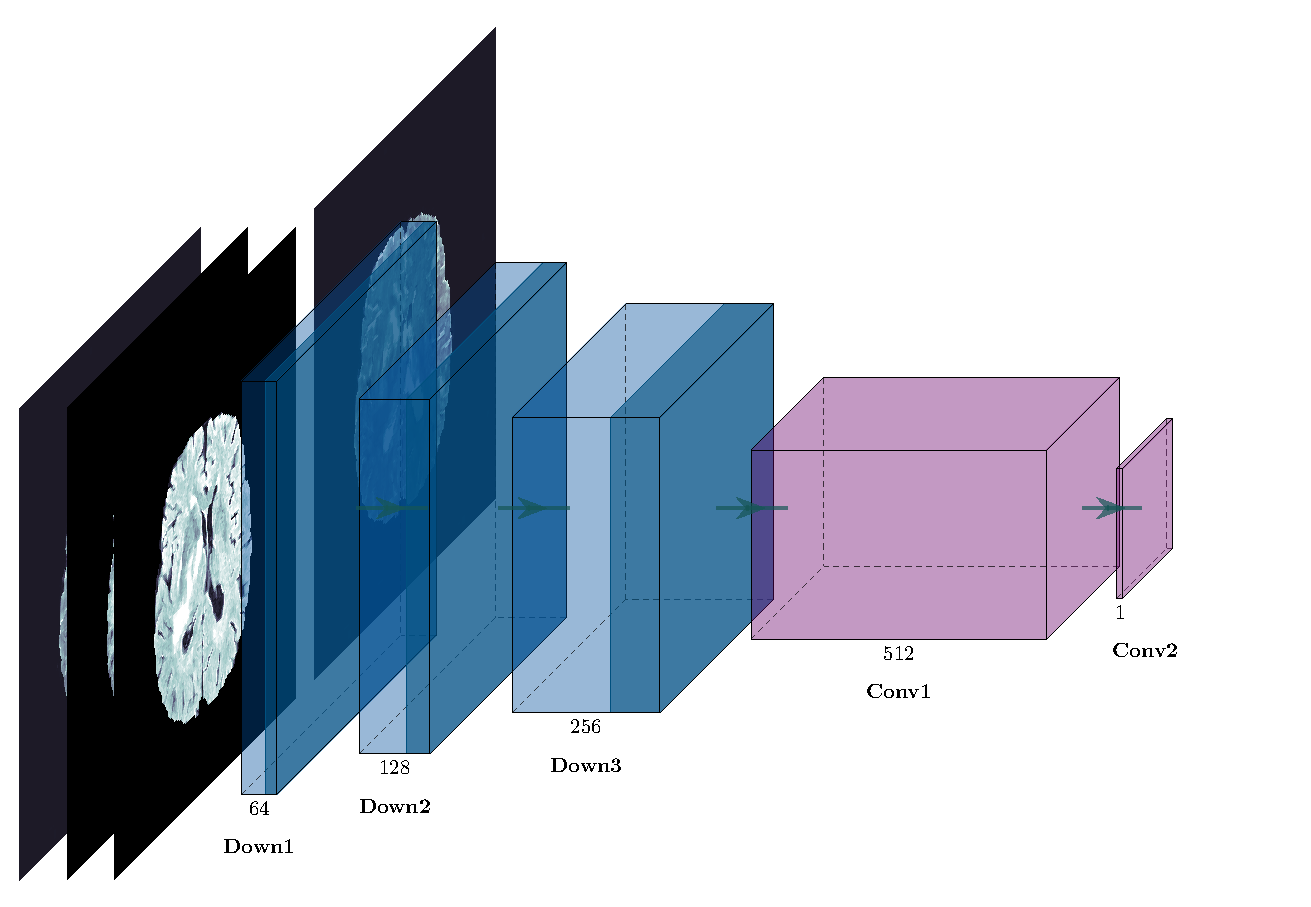
\includegraphics[height=0.335\textheight]{images/MIpix2pix_discriminator.pdf}
\caption[Discriminator architecture from MI-pix2pix]{Discriminator architecture from MI-pix2pix.}
\label{fig:MIpix2pix_discriminator}
\end{figure}



\noindent MI-pix2pix was very useful to understand whether a multi-modal approach can exploit the information coming from different \ac{MRI} sequences in a better way than what is done by pix2pix, since the two \ac{GAN}s share the same architecture and the same layers but receive a different number of images. The results of the comparison are presented in Chapter \ref{cha:5th_chapter}.

\vspace{2mm} %5mm vertical space
As for pix2pix, description of the training used can be found in Subsection \ref{subsec:training_algorithm} while the implementation details are discussed in Subsection \ref{subsec:implementation_details}.

\subsection{MI-GAN}
\label{subsec:mi_gan_architecture}
The third Generative Adversarial Network that we implemented is a multi-modal approach inspired by the work of Anmol Sharma and Ghassan Hamarhneh that in 2019 presented a multi-input multi-output \ac{GAN}, called MM-GAN, that seems to be, to the best of their knowledge, the first method capable of synthesizing multiple missing sequences using a combination of various input sequences (many-to-many) \cite{migan}.

\vspace{2mm} %5mm vertical space
Since the core of this work is on the generation of a single-output image, using different configurations and architecture of \ac{GAN}s, we focused our attention on a modified version multi-input single-output (many-to-one) of MM-GAN, called MI-GAN and implemented also by Sharma and Hamarhneh.

The focus of \cite{migan} was on the many-to-many approach though, and as a consequence many details about the MI-GAN model weren't given: because of this, our model was inspired by the MM-GAN but at the same time it presents some variations that we applied, both to the architecture and to the loss used in the training algorithm (Subsection \ref{subsec:training_algorithm}), in order to obtain a more stable training and satisfiable results in the generated samples.

\vspace{2mm} %5mm verticalspace
The layers that define the architecture of MI-GAN are almost the same proposed in \cite{migan} for the MM-GAN: the only variation applied was the replacement of every layer of Instance Normalization with a Batch Normalization, used also in pix2pix (Subsection \ref{subsec:pix2pix_architecture}) and in MI-pix2pix (Subsection \ref{subsec:mi_pix2pix_architecture}), after observing through various experiments that normalizing the activations of each channel across the whole batch was more effective, in terms of quality in the generated samples, instead of computing the mean/standard deviation and normalizing across each channel in each training image.

\vspace{6mm} 
\noindent\textbf{Generator}

\vspace{2mm}
\noindent The generator is a modified U-Net with concatenated skip connections and the typical U-shape architecture (Figure~\ref{fig:MIGAN_generator}), characterized by two known building blocks: one that downsamples its input and one that, through a transposed convolution, performs an upsampling. 

The \textbf{downsample block} is composed in a similar way to the one used in the previous model, with the addition of a dropout layer at the end of the block.

\begin{itemize}
\item \textbf{Convolution} with kernel size equal to 4 and stride of 2.
\item \textbf{Batch Normalization} in every block beside the first one.
\item \textbf{Leaky ReLU}
\item \textbf{Dropout} with the rate defining the fractions of the input dropped to 0, at each update during training time, set to 0.5. 
\end{itemize}

\begin{figure}[H]
\centering
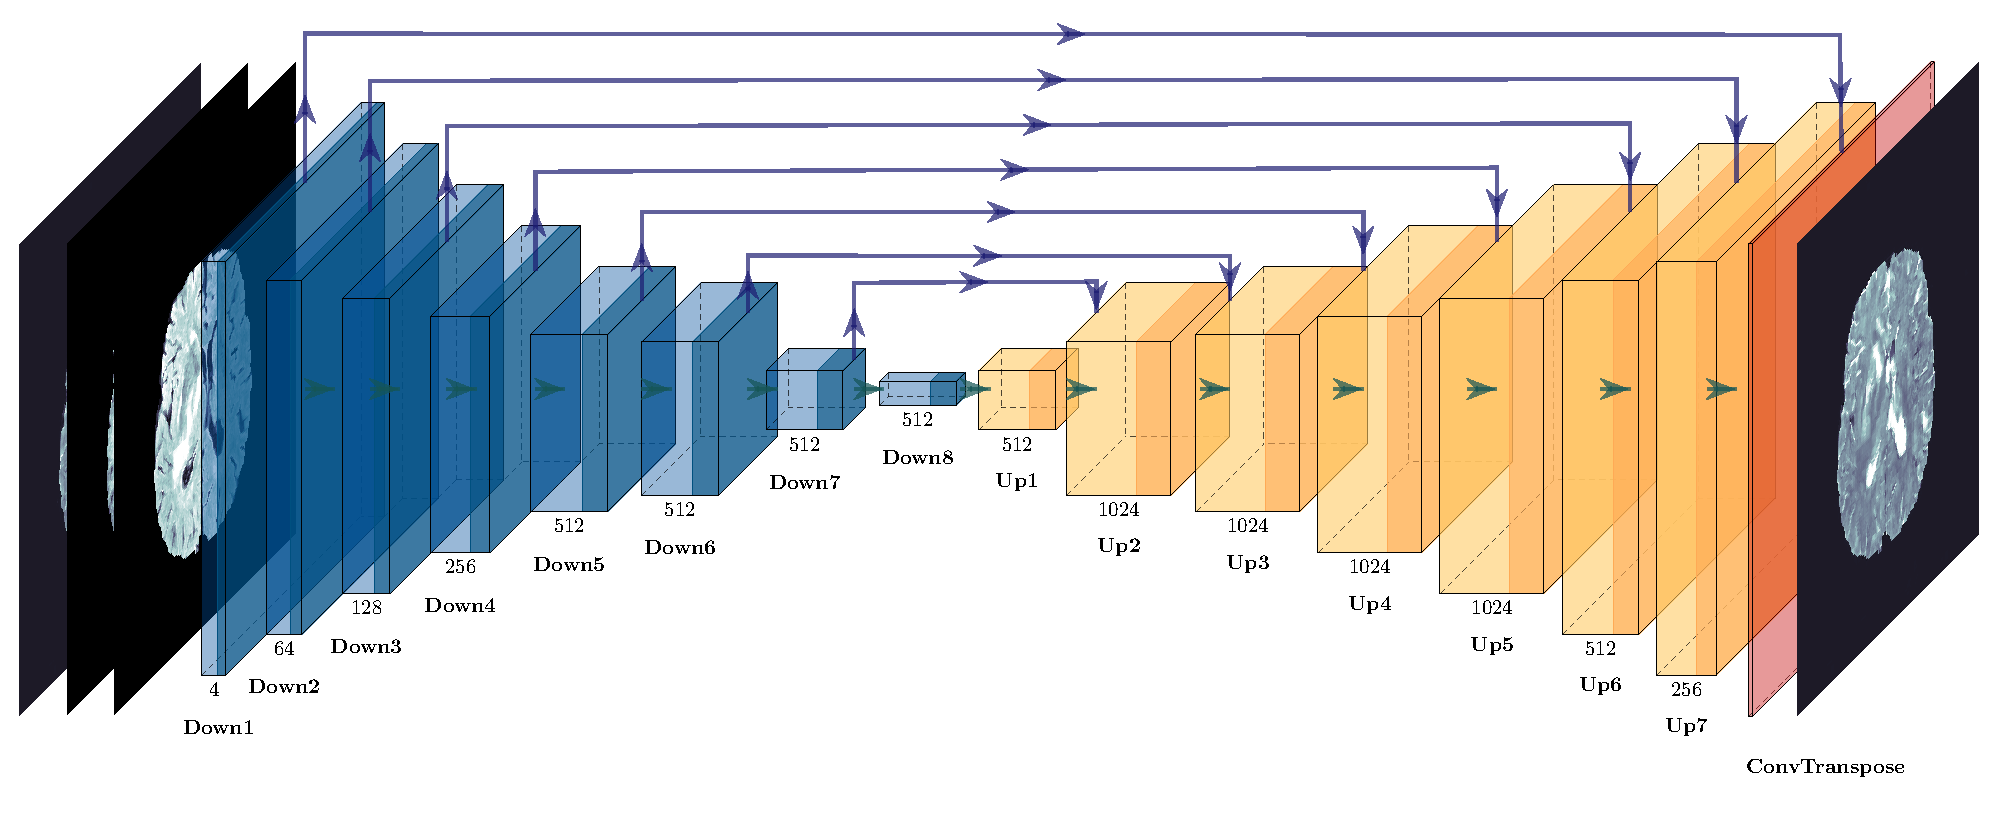
\includegraphics[height=0.263\textheight]{images/MIGAN_generator.pdf}
\caption[Generator architecture of MI-GAN]{Generator architecture of MI-GAN.}
\label{fig:MIGAN_generator}
\end{figure}

The \textbf{upsample block} instead, following the MM-GAN architecture, has the same layers seen in the pix2pix architecture with the difference that the dropout layer is applied after the ReLU activation function:

\begin{itemize}
\item \textbf{Transposed Convolution}
\item \textbf{Batch Normalization}
\item \textbf{ReLU}
\item \textbf{Dropout} (with 0.5 rate) applied to the first three upsample blocks.
\end{itemize}

At the end of the network, after the last upsample block, a transposed convolution with tanh as activation function is used to reduce the feature dimension and to enlarge the spatial dimensions of the image from 128x128 to the final shape of 256x256.

\vspace{5mm} %5mm vertical space
Regarding the problem of how many input and output channels use in the generator, we performed two experiments with the architecture above defined: in the first one, following \cite{migan} and adapting the MM-GAN network from a many-to-many to a many-to-one scenario, we trained a generator to produce 4 different modalities (but only the synthesized image of the missing sequence was used to compute the loss, while the other three were discarded) receiving as input a concatenation of 4 images.
These images given as input, in the case for example of $T_{1}$ missing, were the three remaining modalities \{$T_{2}$, $T_{1c}$, $T_{2flair}$\} and a zero-value image through the channel of the missing sequence (so the channel of $T_{1}$ was obscured).
The second approach we tested was about using a generator with the same input and output shape already used in MI-pix2pix: a single image with shape [32, 256, 256, 1] generated by a model that receives three 32x256x256 different modalities.

\vspace{5mm} %5mm vertical space
The results obtained led us to discard the first solution, probably more functional in a many-to-many scenario, and to choose the second approach that outperformed the other one both in a qualitatively (human perception of quality from the generated samples) and quantitatively (scores from the similarity/error metrics applied to the synthesized images) way.

\vspace{6mm} 
\noindent\textbf{Discriminator}

\vspace{2mm}
\noindent The experiments we did in order to find the best suitable network involved also the Discriminator: with the generator synthesizing 4 images, we implemented the model discussed in \cite{migan} that takes two inputs $X_t$ and $X_i$ and produces one output D($X_t$, $X_i$), each one of these with 4 channels, one per modality: assuming the discrimination of a $T_{1}'$ synthesized scan, the inputs were $X_t$: \{$T_{1}$, $T_{2}$, $T_{1c}$, $T_{2flair}$\} and $X_i$: \{$T_{1}'$, $T_{2}$, $T_{1c}$, $T_{2flair}$\}.

In second experiment, the one with the generator producing only one image, the two discriminator inputs, input and target, had respectively shape [32, 256, 256, 3] and [32, 256, 256, 1] with an output with dimensions equal to 32x15x15x1 (in the discrimination of a $T_{1}'$ scan, the inputs were \{$T_{2}$, $T_{1c}$, $T_{2flair}$\} and $T_{1}'$).
As said before, we choose to use the second solution, over the first one.

\vspace{5mm} %5mm vertical space
The discriminator is a PatchGAN \cite{patchgan} composed by four downsampling steps called \textbf{discriminator blocks}, similar to the ones used by the MM-GAN {\cite{migan}}. Each block contains, in order, the following layers:

\begin{itemize}
\item \textbf{Convolution}, with a number of filters ranging from 64 (first block) to 512 (last block).
\item \textbf{Batch Normalization} applied in the second, third and fourth block.
\item \textbf{Leaky ReLU}
\end{itemize}

At the end of these sequence of blocks, two more layers are applied (Figure~\ref{fig:MIGAN_discriminator}):

\begin{itemize}
\item \textbf{Zero Padding}
\item Final \textbf{Convolution} with kernel size to 4 and strides set to 1.
\end{itemize}

\noindent The description of the training algorithm as well as the loss formulation used by MI-GAN is in Section \ref{sec:training}, while the implementation details are discussed in Subsection \ref{subsec:implementation_details}.

\begin{figure}[H]
\centering
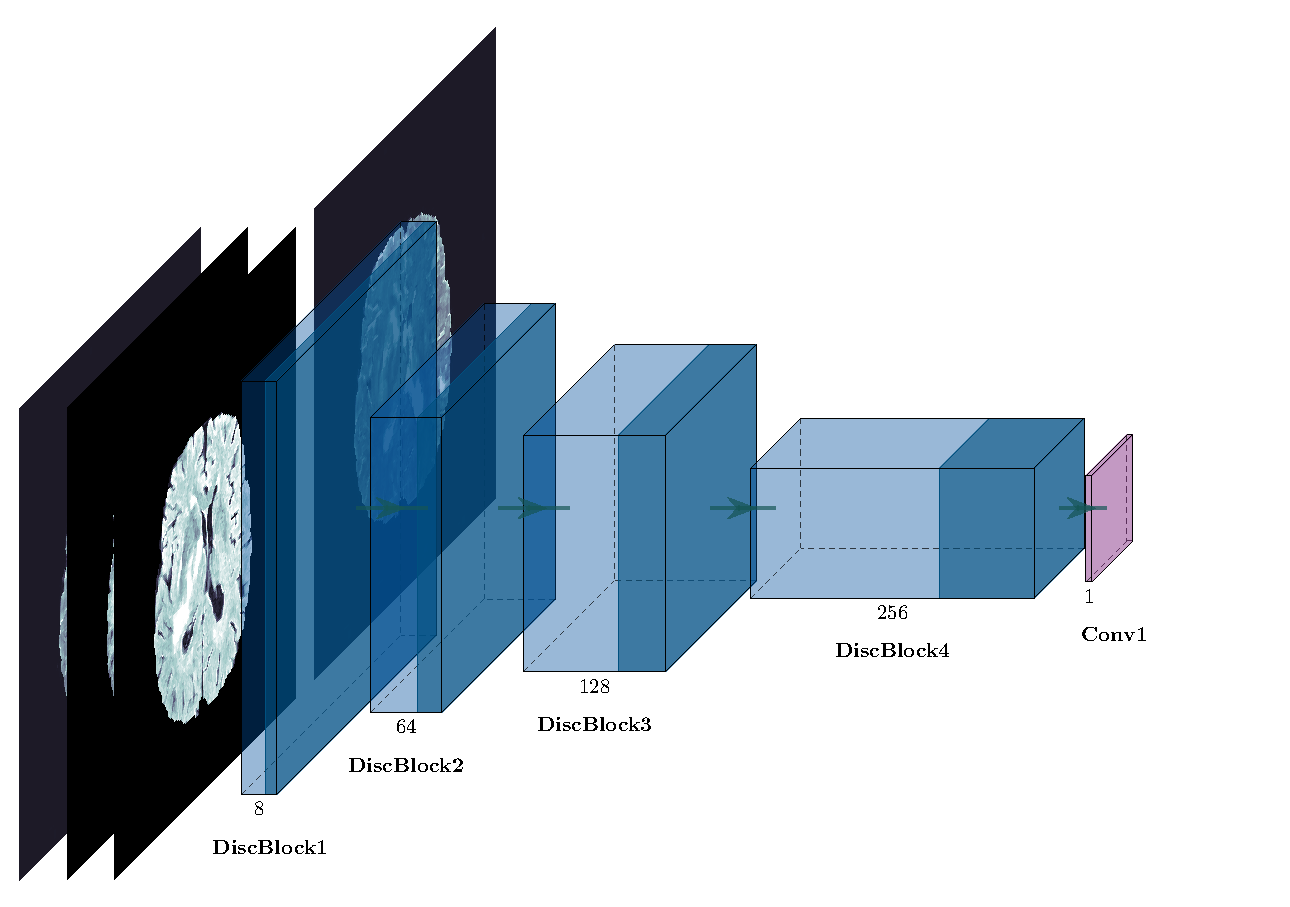
\includegraphics[height=0.335\textheight]{images/MIGAN_discriminator.pdf}
\caption[Discriminator architecture of MI-GAN]{Discriminator architecture of MI-GAN.}
\label{fig:MIGAN_discriminator}
\end{figure}

\section{Training}
\label{sec:training}
In a Generative Adversarial Network, generator and discriminator are trained simultaneously using \textit{Backpropagation}, with D that learns to recognize the true images from the fake ones and G that, based on the feedback received by the first neural network, learns to produce more realistic images in order to be able to fool D. In this adversarial setting, the competing behaviour of one against each other is defined by two different loss functions.

\subsection{Loss Formulation}
\label{subsec:loss_formulation}
The generator loss and discriminator loss used with MI-GAN (\ref{subsec:mi_gan_architecture}) are the ones proposed in \cite{pix2pix} and defined as follows: 

\begin{equation} \label{eq:losses_migan}
\begin{gathered}
L_G\leftarrow \lambda\mathcal{L}_{1}(G(x), y) + (1 - \lambda) \mathcal{L}_{2}(D(x, G(x)), L_{ar})  \\
L_D \leftarrow \mathcal{L}_{2}(D(x, y), L_{ar}) + \mathcal{L}_{2}(D(x, G(x)), L_r) 
\end{gathered}
\end{equation}

where $x$, the input, is a concatenation of three sequences while $G(x)$ represents the prediction generated by the \ac{GAN}.
$L_{ar}$ is a dummy ground truth tensor that is used by the generator loss to fool the discriminator by setting all the entries to one, in such a way that G is encouraged to generate modalities that can fool D.

$\mathcal{L}_{2}$ is the L2 norm (also known as mean squared error) while $\mathcal{L}_{1}$ instead is the mean absolute error (L1 norm) that is useful to the generated image because it allows to become structurally similar to the target image. This term was chosen as reconstruction loss term because of its ability to prevent too much blurring, as compared to using a L2 loss \cite{migan}.
$L_r$ is instead a tensor with its entries equal to zero, useful for D to distinguish the fake samples (associated to 0, by using $L_{r}$) from the true samples (associated to 1 through $L_{ar}$).

\vspace{5mm} %5mm vertical space
Pix2pix (\ref{subsec:pix2pix_architecture}) and MI-pix2pix (\ref{subsec:mi_pix2pix_architecture}) share the same objective function (Eqn.~\ref{eq:final_objective}), since they have an identical architecture and the only difference between the models is in the number of inputs that their generator can receive.

In the implementation of these two networks, we applied the same losses that are used in \cite{pix2pix_implementation}, similar to the ones adopted in the MI-GAN training algorithm: here, a binary crossentropy is used instead of the L2 term. 

The $L_D$ of pix2pix and MI-pix2pix is computed as the sum between the binary crossentropy of $(D(x,y), L_{ar})$ and the one of $D((x, y'), L_{r})$ where $y'$ is the generated image.
$L_G$, on the other hand, contains the reconstruction term between $y$ and $y'$, multiplied by an hyper parameter lambda and summed to the binary crossentropy of $D((x, y'), L_{r})$.

\subsection{Training Algorithm}
\label{subsec:training_algorithm}
Due to some implementation needs and to be able to define our own metrics (Section \ref{sec:evaluation_metrics} for details) and losses, we wrote a custom train step (where is contained the update of the weights) as well as evaluation loops instead of using the built-in training optimized by \textit{Tensorflow}. The two approaches work strictly in the same way across every kind of \textit{Keras} model, but implementing everything from scratch allowed us to have a lower-level training and full control on the evaluation step, as well as the possibility to being able to retrieve all the gradients of the trainable weights of a layer with respect to the loss.  

For implementing the training algorithm we followed the algorithm applied in \cite{pix2pix_implementation}, which uses \textit{Adam} \cite{kingma2014adam}, an adaptive learning rate method, as optimizer for both the networks.

\vspace{5mm} %5mm vertical space
During the training of our models, we didn't make use of the regularization technique called \textit{Early Stopping}, used to prevent overfitting in many \ac{DL} methods. This technique is based on the idea of stopping the training procedure before the model starts to overfit, by looking at the performances on the validation set, in particular at the validation loss: when its value, after an initial improvement of the learner's ability to generate/predict/classify, starts to increase, it means it is probably the right moment to stop the training because the models is incurring into a larger generalization error. In our case though, we observed that, often, after an abrupt increase of one of the two losses, the networks after few epochs were returning to a stable training level, without the need of killing the procedure and restarting again from the beginning. 

\begin{figure}[H]
\centering
\includegraphics[height=0.331\textheight]{images/loss_behaviour2.pdf}
\caption[Validation loss during MI-GAN training]{Typical behaviour of the validation losses through the epochs of MI-GAN training.}
\label{fig:loss_behaviour}
\end{figure}

Furthermore, our Generative Adversarial Networks continued to improve the overall quality of their generated image even if their losses values, the indicators used to understand when we should stop, had been stable for 10, 20, even 30 epochs: \ac{GAN}s took long time to train and long time to show some progress in the synthesized samples, that's why it was important to wait for a while before killing the training. The only exception is represented by the case in which the loss went rapidly to 0, sign that something wasn't working in the proper way and that the network had incurred in a failure to converge, that can happen for example when the discriminator loss drops to 0 because it is learning more rapidly with respect to the generator.

\vspace{5mm}
Figure~\ref{fig:epochs_behaviour} illustrates the differences between the original $T_{1c}$ slice and its prediction, from MI-GAN, after 5 and 20 epochs of training: it shows how much a \ac{GAN} can improve the quality of the generated images, adding low-level details and reducing the overall blurriness, even when the losses, both in the generator and in the discriminator, are not improving over time (Figure~\ref{fig:loss_behaviour}): proof that, during training, a visual understanding is much more meaningful than just looking at the values of the losses.


\begin{figure}[H]
\centering
\includegraphics[height=0.56\textheight]{images/t1c_through_epochs.pdf}
\caption[$T_{1c}$ predictions from MI-GAN]{Prediction of $T_{1c}$ slices on the validation set, using MI-GAN.}
\label{fig:epochs_behaviour}
\end{figure}
\newpage
\subsection{Implementation Details}
\label{subsec:implementation_details}

The hyperparameters used are the learning rate $\alpha$ set to 0.0002 and the exponential decay rate for the 1st moment estimates $\beta_1$ equal to 0.5 while the one for the 2nd moment estimates ($\beta_2$) was left to the default value of 0.999.

$\lambda$ has a value of 100 in the generator loss of pix2pix and MI-pix2pix, while is set to 0.9 in the loss of the MI-GAN generator. 
The MI-GAN discriminator loss instead is multiplied by 0.5, choice motivated by the need to slow down the rate at which D learns compared to G.

\vspace{5mm} %5mm vertical space
Furthermore, the transposed convolution layers in the generators architectures (whose shapes are summarized in Table~\ref{tab:resume_architectures_generators}) as well as the convolutions used by both generators and discriminators (Table~\ref{tab:resume_architectures_discriminators}) have a variable number of filters with dimension 4x4 and with kernel weights initialized using a normal distribution with 0 mean and standard deviation equal to 0.05.

\begin{table}[htbp!]
\centering
\begin{tabular}{ccc}
\toprule
Model & Inputs & Output\\
\midrule
pix2pix Generator & [32, 256, 256, 1] & [32, 256, 256, 1]\\
MI-pix2pix Generator & [32, 256, 256, 3] & [32, 256, 256, 1]\\
MI-GAN Generator & [32, 256, 256, 3] & [32, 256, 256, 1]\\
\bottomrule	
\end{tabular}
\caption[Generators input and output shapes used during training]{Generators input and output shapes used during training. 32 is the batch size we choose to use. The last input dimension is the number of channels, so it represents how many modalities can be fed to the model.}
\label{tab:resume_architectures_generators}
\end{table}

\begin{table}[H]
\centering
\begin{tabular}{ccc}
\toprule
Model & Inputs & Output\\
\midrule
pix2pix Discriminator & [32, 256, 256, 1],[32, 256, 256, 1] & [32, 30, 30, 1]\\
MI-pix2pix Discriminator & [32, 256, 256, 3],[32, 256, 256, 1] & [32, 30, 30, 1]\\
MI-GAN Discriminator & [32, 256, 256, 3],[32, 256, 256, 1] & [32, 15, 15, 1]\\
\bottomrule	
\end{tabular}
\caption[Discriminators input and output shapes used during training]{Discriminators input and output shapes used during training.}
\label{tab:resume_architectures_discriminators}
\end{table}

Python 3.6.9 is the main programming language of our work. We used \cite{pix2pix_implementation} as reference for the implementation of the pix2pix model that, as MI-pix2pix and MI-GAN, was built using mainly the library of Tensorflow 2.1.0. For our experiments we used \href{https://colab.research.google.com}{Google Colaboratory}, a hosted Jupyter notebook service, that offers free usage of its computing hardware consisting of a Tesla P100-PCIE-16GB GPU with 26 GB of RAM available and an Intel(R) Xeon(R) CPU @ 2.30GHz.
\newpage
\section{Evaluation Metrics}
\label{sec:evaluation_metrics}
In \autoref{subsec:training_algorithm} we discussed about how much is important to evaluate an image in a qualitatively way, by looking not only at the losses values reached by the networks through the epochs in the training phase but also at the quality of the generated samples. 
Beside the qualitative measure though, it was necessary to define some quantitative metrics that were able to understand how much error and similarity there were between our prediction and the original image. 

\vspace{5mm} %5mm vertical space
These metrics resulted particularly useful during training when there wasn't any visible difference in the quality of the synthesized modalities between two epochs as well as, on the other hand, human perception was very effective in the cases of images, from different epochs, with almost same values but with a clear difference in low-level details that the metrics couldn't capture.

\subsection{Evaluation of the Whole Image}
\label{subsec:eval_overall_area}
The first metrics we implemented were the ones to evaluate the whole area of the images produced by the \ac{GAN}s. In order to obtain results as more accurate as possible, we proceeded to crop and normalize both the prediction and the original image: we center-cropped the generated images of size 256x256 to the dimensions of 155x194, after calculating the largest bounding box able to contain each brain of the dataset \cite{migan}. 

This was motivated by the fact that computing, for example, the similarity between two images padded to have compatible size with the input of the networks returns a much higher value than the one obtained comparing two 155x194 slices: an high value due to the presence of many black pixels that risks to bias the performances on the metrics (Figure~\ref{fig:before_after_crop}).

\begin{figure}[H]
  \centering
  \subfloat{\includegraphics[height=0.24\textheight]{images/256x256.pdf}
  \label{fig:f1}}
  \hspace{1.6cm}
  \subfloat{\includegraphics[height=0.145\textheight]{images/155x194.pdf}\label{fig:f2}}
  \caption[$T2$ slice before and after crop to 155x194]{$T2$ slice before and after crop to 155x194, applied to remove as many not relevant pixels as possible before the calculation of the metrics.}
  \label{fig:before_after_crop}
\end{figure}

\vspace{5mm} %5mm vertical space
In order to obtain consistent results during the comparison and avoid to compute a metric between an original image that has intensity values ranging from 0 to 1 and a predicted image with a different range, happening especially during the evaluation of the model in the first epochs of the training (while at the end of the training the \ac{GAN} learns to synthesize images that lie in the same normalized range of the input image), we proceeded to apply a scaling.

The transformation applied to the original image and to its prediction is a \textbf{mean normalization}, whose formula, taken from \cite{mean_norm}, is the following:

\begin{equation} \label{eq:mean_normalization}
x' = \dfrac{x - \mathrm{average(x)}}{\max(x) - \min(x)}
\end{equation}

where \textit{x} is the original value, \textit{x'} is the normalized value. This method, similar to the min-max, allows the pixels to have approximately zero mean and dynamic range equal to 1. 

Differently from the normalization done, in the preprocessing step (Section \ref{sec:preprocessing}), to the whole volume, here the transformation is applied with respect to the slice (the min and max values are respectively the minimum and maximum intensity values of the slice, not of the whole volume). We didn't normalize with respect to the volume because our \ac{GAN}s are trained to predict a single image based on a single slice: therefore we considered this approach as a better method to evaluate our predictions.

%The metrics implemented to evaluate the overall area of the brain consider in the calculations not only the pixels relative to the brain but also the ones with zero-value: even if removing all the black pixels wouldn't have been wrong, we preferred the first approach since the \ac{GAN} generates 

\vspace{6mm} 
\noindent\textbf{Mean Squared Error}

\vspace{2mm}
\noindent Mean Squared Error (MSE), one of the metrics that we implemented, allows to estimate the error between its inputs. More specifically, MSE measures the average squared difference between the estimated pixels values and the intensity values belonging to the true image. It is computed as:

\begin{equation} \label{eq:mse}
MSE =  \frac{1}{N} \sum_{i=1}^{N} (y_i - y'_i)^2
\end{equation}

where $y_i$ is the original image while $y'_i$ is the synthesized image. 

To implement it, we used a function from the library of Tensorflow that computes a MSE per each pixel in the image (that is the same of doing just a squared difference between the true pixel and the predicted pixel, since N = 1). The function returns a matrix 155x194, whose values are then averaged to obtain the final mean squared error between $y_i$ and $y'_i$.

\newpage
\noindent\textbf{Peak Signal-to-Noise Ratio}

\vspace{2mm}
\noindent Peak signal-to-noise ratio, often abbreviated PSNR, is a metric that computes, in decibels (dB), the ratio between the maximum intensity value allowed in the image \cite{psnr} and the MSE and is defined as:

\begin{equation} \label{eq:psnr}
PSNR =  10\log_{10} \frac{I^2_{max}}{MSE}
\end{equation}

where $I_{max}$ is the dynamic range that corresponds to the maximum intensity value of the image when its range is [0, 1].
The higher the PSNR, the better is the quality of the predicted image, since the ratio has a measure of error, the MSE, as denominator. For the implementation of this metric we used a built-in function from Tensorflow that receives two images and directly computes the PSNR value.

\vspace{6mm} 
\noindent\textbf{Structural Similarity}


\vspace{2mm}
\noindent This metric is defined as the structural similarity (SSIM) index between two images, designed to improve on traditional metrics such as Mean Squared Error and Peak Signal-to-Noise Ratio. 
SSIM ranges from 0 to 1 and is a metric that doesn't compare the images just on a single statistic: its value of similarity is based on different factors such as the luminance, the contrast and the structure. Furthermore, the structural similarity is applied locally over the image due to the fact that pixels spatially close are the ones with stronger inter-dependencies, somehow similar to the way in which human perception works. SSIM is computed as:

\begin{equation} \label{eq:ssim}
SSIM =  \frac{(2\mu_x + \mu_y + c_1)(2\sigma_{xy} + c_2)}{(\mu^2_x + \mu^2_y + c_1)(\sigma^2_x + \sigma^2_y + c_2)}
\end{equation}

where $x, y$ are the two images to be compared, $\mu$ is the mean intensity, $\sigma^2$ the variance of the image and $\sigma_{xy}$ the covariance of $x, y$.

\vspace{5mm} %5mm vertical space
For calculating this metric we used the implementation provided by the Tensorflow library which in turn is based on the standard SSIM implementation from \cite{ssim}. The only parameter that we needed to specify was the dynamic range of the images (difference between the max and min allowed values), that in our case, thanks to the mean normalization, is equal to 1. 

The SSIM reported in Chapter \ref{cha:5th_chapter} are obtained by computing the mean and standard deviation over all the SSIM values calculated by comparing each original image in the test test with its prediction. 

\subsection{Evaluation of the Tumor Area}
\label{subsec:eval_tumor_area}

The most relevant part of the brain, to us and in general to the doctors that have to make a diagnosis, is the tumor. Because of this we implemented three more ways in which we could evaluate the results of our predictions, not anymore by looking at the whole brain area but by focusing on the tumor. 

The exact information of which pixels belong to the tumor and which do not is contained in the \textit{Ground Truth} volumes that show the segmentation of the malignant area of the brain.

\vspace{6mm} 
\noindent\textbf{MSE and PSNR} 

\vspace{2mm}
\noindent To compute the performances on the tumor area we implemented a modified version of the metrics used to evaluate the whole area: MSE and PSNR.
To do this, we had first to use the ground truth as a mask to isolate the interested area by setting to 0 all the pixels belonging to the healthy part of the brain.
Figure~\ref{fig:brain_masked} illustrates the result obtained by masking a $T_{2flair}$ slice with its ground truth.

\begin{figure}[H]
\centering
\includegraphics[height=0.30\textheight]{images/brain_tumor_masked.pdf}
\caption[$T_{2flair}$ slices masked with the ground truth]{$T_{2flair}$ slices and their masked versions, using the ground truth.}
\label{fig:brain_masked}
\end{figure}

After scaling with mean normalization (\ref{eq:mean_normalization}) and masking both the original image and the predicted missing modality with the ground truth, we proceeded to measure the quality of the images with the modified versions of MSE and PSNR.

\vspace{5mm} %5mm vertical space
The idea was to modify the MSE (and so the PSNR, that depends on the MSE) by including in the calculation only the pixels belonging to the tumor area, so without considering the pixels corresponding to the back pixels in the ground truth image.

It was necessary to not consider all these black pixels because they would have affected (and boosted) the metrics of similarity, by reaching higher values, as well as the error metrics, by dropping significantly to values close to 0.

We then computed the MSE between the masked images (target masked and prediction masked) by dividing the squared difference by the number of pixels in the ground truth with value different from 0, instead of dividing by the total number of pixels in the whole image. It was sufficient to apply only this slightly variation to the MSE Formula (\ref{eq:mse}), since the squared difference value wasn't affected by the presence of the black pixels: both the masked images had zero intensity in the dark area, resulting in a difference of values equal to 0.

\vspace{5mm} %5mm vertical space
It is also important to highlight that, even if every patient has a tumor, not all the slices extracted from a volume contain a malignant area. Because of this, we didn't include in the calculations the slices whose masked images were completely black, since we are interested in evaluating only the generated area on the tumor: keeping all the masked slices would have boosted, again, the metrics.

\vspace{6mm} 
\noindent\textbf{Dice Similarity Coefficient}

\vspace{2mm}
\noindent To understand the quality of the generation process, beside the human perception and the other quantitative metrics implemented, we proceeded to evaluate our generated images using segmentation models that extract the tumor area from the synthesized missing modalities. 
In particular, we tested the result of the $T_{2flair}$ segmentation model from \cite{giacomello2019brain} using as input the $T_{2flair}$ predictions (with dimensions 256x256) obtained from our trained models (pix2pix, MI-pix2pix and MI-GAN).

\vspace{5mm} %5mm vertical space
The metric we implemented to evaluate the tumor segmentation model is the Dice similarity coefficient (DSC), also known as Sørensen–Dice coefficient, that measures the similarity between two images. DSC ranges from 0 to 1 and is defined as:

\begin{equation} \label{eq:dsc}
DSC =  \frac{2TP}{2TP + FP + FN}
\end{equation}

where TP (True positives) represents the number of pixels in the segmentation image correctly classified as belonging to the tumor while FP (False positives) is the number of pixels misclassified as positive. FN (False negatives) is instead the number of positive pixels in the ground truth that are classified as negative in the segmentation.
To implement this metric, we first counted the TP, FP, FN per every subject and from these values we calculated the DSC with respect to the volume, using \ref{eq:dsc}, and then we averaged the computed values of the 28 volumes (from the test set) to obtain the final score, reported in Chapter \ref{cha:5th_chapter}. Figure~\ref{fig:segmentation_example} shows the segmentation obtained from $T_{2flair}$ slices using a segmentation model \cite{giacomello2019brain}: the DSC is computed between the ground truth and the segmentation.

\begin{figure}[H]
\centering
\includegraphics[height=0.36\textheight]{images/segmentation_example.pdf}
\caption[Comparison between Ground Truths and Segmentations]{Comparison between Ground Truths and segmentations of $T_{2flair}$ slices obtained using the segmentation model from \cite{giacomello2019brain}.}
\label{fig:segmentation_example}
\end{figure}

\section{Summary}
\label{sec:4th_section_summary}
In this chapter we first discussed about the input pipeline optimization of our models. We proceeded then to present a detailed description about the architectures of the models we implemented: pix2pix, MI-pix2pix, MI-GAN.

We gave an overview of the training algorithm, of the losses used in the update step and the implementation details of this work in order to allow the reproducibility of our results.

At the end of the chapter is described how we evaluated the synthesized missing modalities obtained from the \ac{GAN}s in order to measure, as accurately as possible, the quality of the generation in both the tumor area and the whole area of the brain.